\documentclass{article}

\usepackage[english]{babel}
\usepackage[utf8]{inputenc}
\usepackage{graphicx}
\usepackage{amsmath,amssymb}
\usepackage{subcaption}
\usepackage{hyperref, url}
\usepackage[table,xcdraw]{xcolor}
\usepackage[font=small,labelfont=bf]{caption}
\usepackage{hyperref}
%\parindent 0mm
%\parskip mm

% add your name and student number in parenthesis
\title{TCGA Liver cancer survival analysis of expressed gene transcript\vspace{-1ex}}
\author{Sailendra Pradhananga (sailendra.pradhanaga@scilifelab.se)\\ 
			Project Report:Algorithms in Bioinformatics\\ 
			KTH Royal Institute Of Technology}
			

\begin{document}

\maketitle
\section{Introduction}

Survival analysis are statistical toolkits that are used to analyzing the outcome of variables based on time period of event occurrence. The event could be either be death, outbreak of disease or failure of automobile parts which are then followed specified time period in days, weeks or years. 

The survival analysis datset consists of two kinds of response variables:first, the time to event and second the information on event occurrences. Various parametric and semi/non - parametic methods are developed to evaluate time based response of event. Kaplan Meier method or regression model such as cox proportional hazards evaluates two functions that is  survival function and hazard function  based on these response variables with other categorical and numerical dependent variables. The survival function gives the probability  for each time-points of surviving up to that events while hazard function whether the event has occurred or not  given the individual survival. The main aim of these type of analysis is find the relationship between the survival time and variables under study such as drugs, gene expression, treatment either with or independent on different covariates such as age, gender, race.

In the current project, using publicly available high-throughput RNA expression of liver cnacer tumor sample, subsequent phenotype characterstic and time of survial information, we aimed at evaluating survival analysis of each gene transcipt. The raw data were subsequently preprocessed, fitted into cox propotional regression hazard model and each gene transcript was evaluated for potential prognostic marker for survial of patients at 5\% and 1\% false discovery rate.
 

\section{Material and Method}

	\subsection{Acquistion of raw TCGA Dataset}
The  TCGA dataset for the analysis was download from \url{http://kaell.org/files/survivalLIHC.txt} website. As already stated in the project guidelines, these are liver cancer patient expression data from the sequenced liver tumor. The  dataset consists of both categorical features and numerical data of gene expression dataset.Therefore, there are few additional features of each cancer patient including ethnicity, sex , age ,iver cancer sub-types and survival time. This raw dataset were first read into python notebook as pandas data frame  as done in  jupyter notebook, \url{https://github.com/sailepradh/prj_algo_bioinfo/blob/master/notebook/TCGA_project.ipynb}.  Additional exploratory analysis was done in the notebook itself.

	\subsection {Preprocessing of Dataset}
The provided raw dataset consists of detailed information of patient phenotypes, howver, survival analysis model are unable to process these information. Hence these information needed to be catagorically coded before proceding into actual analysis. Phenotypic features of cancer patient sample such as gender, race, status, liver cancer subtypes were coded into different codes. Furthermore, gene transcripts which lacked expression data in atleast one of patients were removed from further analysis as these feature will unable to provide prognostic marker information.

	\subsection{Cox proportional Hazard model}
	 Cox proportional hazards model are regression model used to relate the survival time with one or more predictor catagorical and quantitative variabeles.As our goal in current project is test expression of each transcript as prognostic marker of survial, Cox proportional hazard model aptly fits the requirement. Each gene transcript expression values are modeled aganist the survival time and survival status for patient sample. To this end, we specifically used the Cox regression hazard model implementation in python from lifelines \cite{lifelines} module. Based on proportional hazard model we get a hazard function,survival probability and p-value estimates of gene transcript as prognostic marker. However we fount that not all the gene transcripts were fitted into the Cox survival model ,thus we excluded to get final list of pvalues for each transcripts.
	 
	\subsection {Multiple testing correction}
	In order to control the false postive rate due to multiple feature testing, we implemented Storey and Tibshirani \cite{storey2003statistical} $q$ value estimates based on cox modeled p-value of gene transcript. As discussed in earlier exercises we have  implemented multiple testing correction Furthermore, we estimated $\hat {\pi_0}$ from differnt $\lambda$ values in order to make q value estimates  of $i$th significant feature. These implementation were made on python and can be observed in associated notebook.

 \section{Result}
	\subsection {TCGA Liver Cancer cohort characterstics}
 
The cancer cohort consists of different phenotypic features such liver cancer types, age, gender, which are further summarized in table~\ref{tab:table1} . Importantly, the important dependent variable is the status of an patient cohort  and the  living days which is the measure of the time of survival.. The average living days for alive  patient cohort is  896.80 while for dead sample cohort is 655.21 with pvalues $< 0.001$ as figure~\ref{fig:status_livingdays}
 
 \begin{table}[h]
\centering
\scalebox{0.65}{
	\begin{tabular}{|l|l|}
	\hline
		\multicolumn{2}{|l|}{\cellcolor[HTML]{96FFFB}{\color[HTML]{FE0000} Summary statistics of TCGA liver cancer cohorts}}                                                                                                                                 	\\ \hline
		\multicolumn{2}{|c|}{Gender}                                                                                                                                                                                                                         	\\ \hline
			\begin{tabular}[c]{@{}l@{}}male\\ \\ female\end{tabular}                                                                                                       & \begin{tabular}[c]{@{}l@{}}245\\ \\ 		119\end{tabular}                               \\ \hline
		\multicolumn{2}{|c|}{Race}                                                                                                                                                                                                                           \\ \hline
			\begin{tabular}[c]{@{}l@{}}white\\ asian\\ black or african american\\ not reported\\ american indian or alaska native\end{tabular}                             & \begin{tabular}[c]{@{}l@{}}182\\ 154\\ 17\\ 10\\ 1\end{tabular}                    \\ \hline
		\multicolumn{2}{|c|}{Liver cancer stage}                                                                                                                                                                                                             \\ \hline
			\begin{tabular}[c]{@{}l@{}}stage i\\ stage ii\\ stage iiia\\ not reported\\ stage iiic\\ stage iiib\\ stage iii\\ stage ivb\\ stage iv\\ stage iva\end{tabular} & \begin{tabular}[c]{@{}l@{}}170\\ 83\\ 63\\ 24\\ 9\\ 8\\ 3\\ 2\\ 1\\ 1\end{tabular} \\ \hline
		\multicolumn{2}{|c|}{Status}                                                                                                                                                                                                                         \\ \hline
		\begin{tabular}[c]{@{}l@{}}alive\\ dead\end{tabular}                                                                                                            & \begin{tabular}[c]{@{}l@{}}234\\ 130\end{tabular}                                  \\ \hline
	\end{tabular}}
\caption{Summary Statistics of TCGA liver cancer cohort \tiny}
\label{tab:table1}
\end{table}

\begin{figure}[tbh]
    \centering
      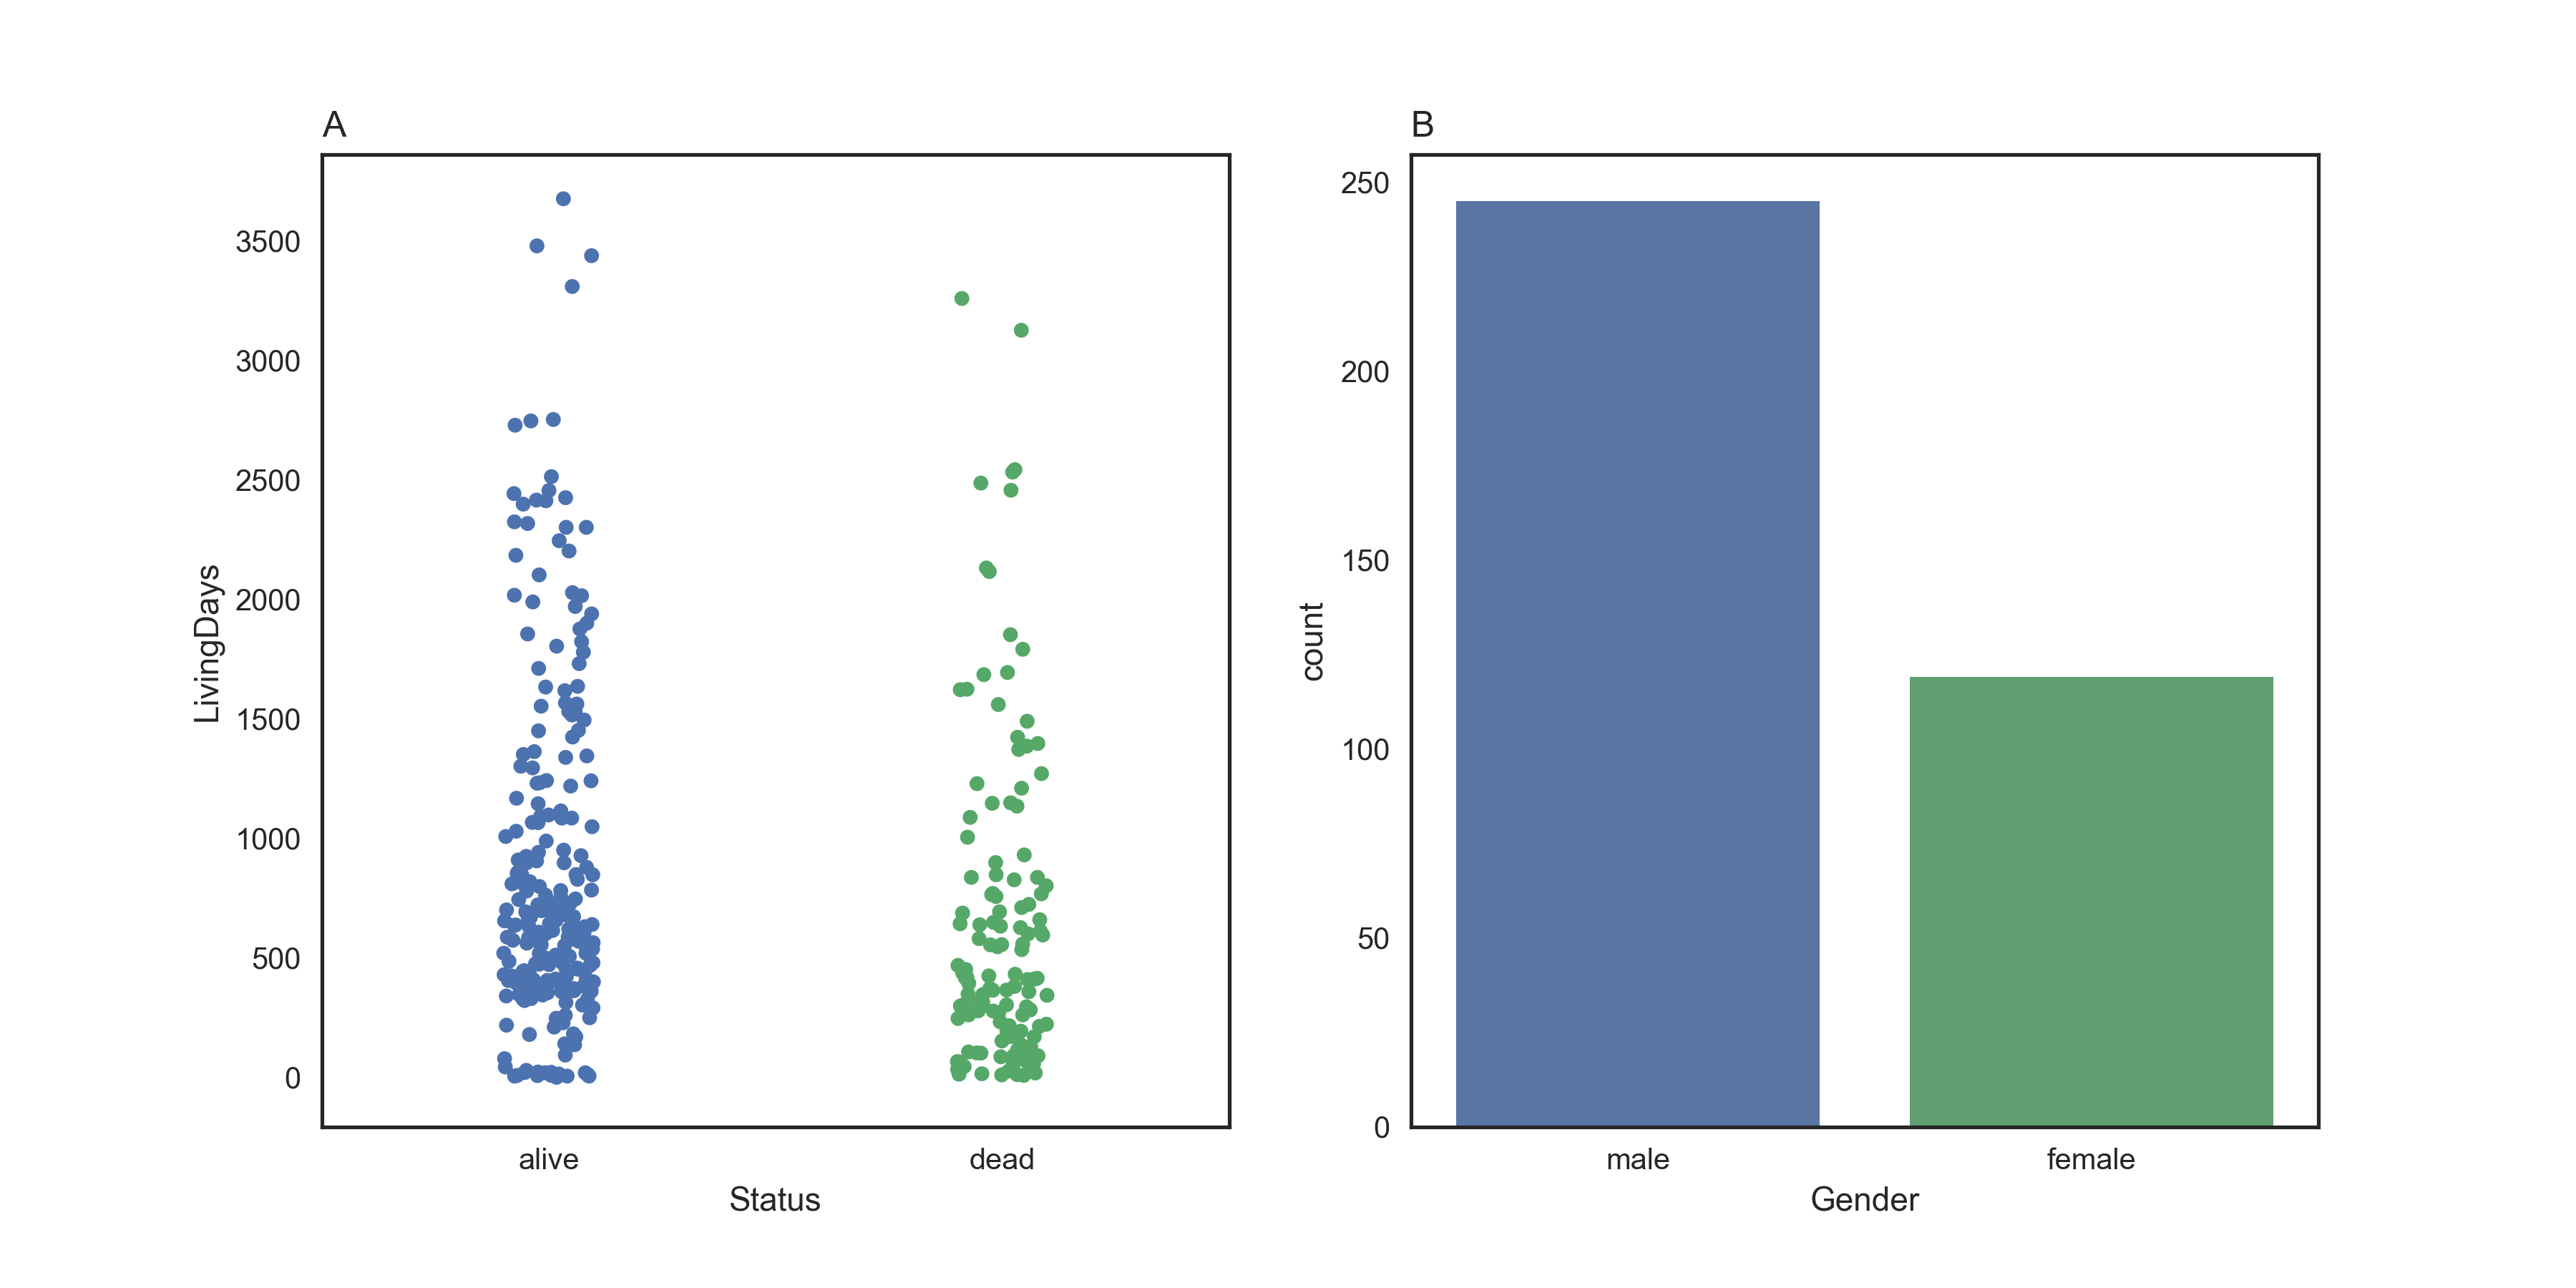
\includegraphics[width=0.75\textwidth]{Genderandstatus.png}
    \caption{A) Number of alive and dead patients in the liver cancer cohort, the number of alive patients are nearly twice as many as dead patients. B) Distribution of living days in two status group , alive and dead.\tiny}
    \label{fig:status_livingdays}
\end{figure}

	\subsection {Gene expression survival analysis with Cox regression model }
	
	The survival analysis requires the time period for the event to occur (in our case death). Thus , in liver cancer cohort variable living days was taken as time variable with status as hazard event. However, other variables had $NA$ available  some categorical features so these were not taken into consideration while building Cox regression hazard model implementation in lifeline module in python. Each transcript was taken as dependent variables in the model which gave us survival probabilities and cumulative hazard estimates for each transcript as shown in the figure~\ref{fig:Baseline_hazard_and_survival}. However not all the gene transcript ran into the model as these gene expression were spares and had missing expression data. These 130 features were excluded from the current analysis.  The cox regression model was run in 19219 gene transcripts completely which gave us hazard, survival function. These estimates provided the p-values as the measure of the significance of gene expression as prognostic marker for  liver cancer survival. Out of 19219 gene expression $6032$ gene expression was considered significant at p-value $< 0.05$. However these are raw p-value without taking into account Cox regression model was run for 19219 features.   
	
\begin{figure}[tbh]
    \centering
      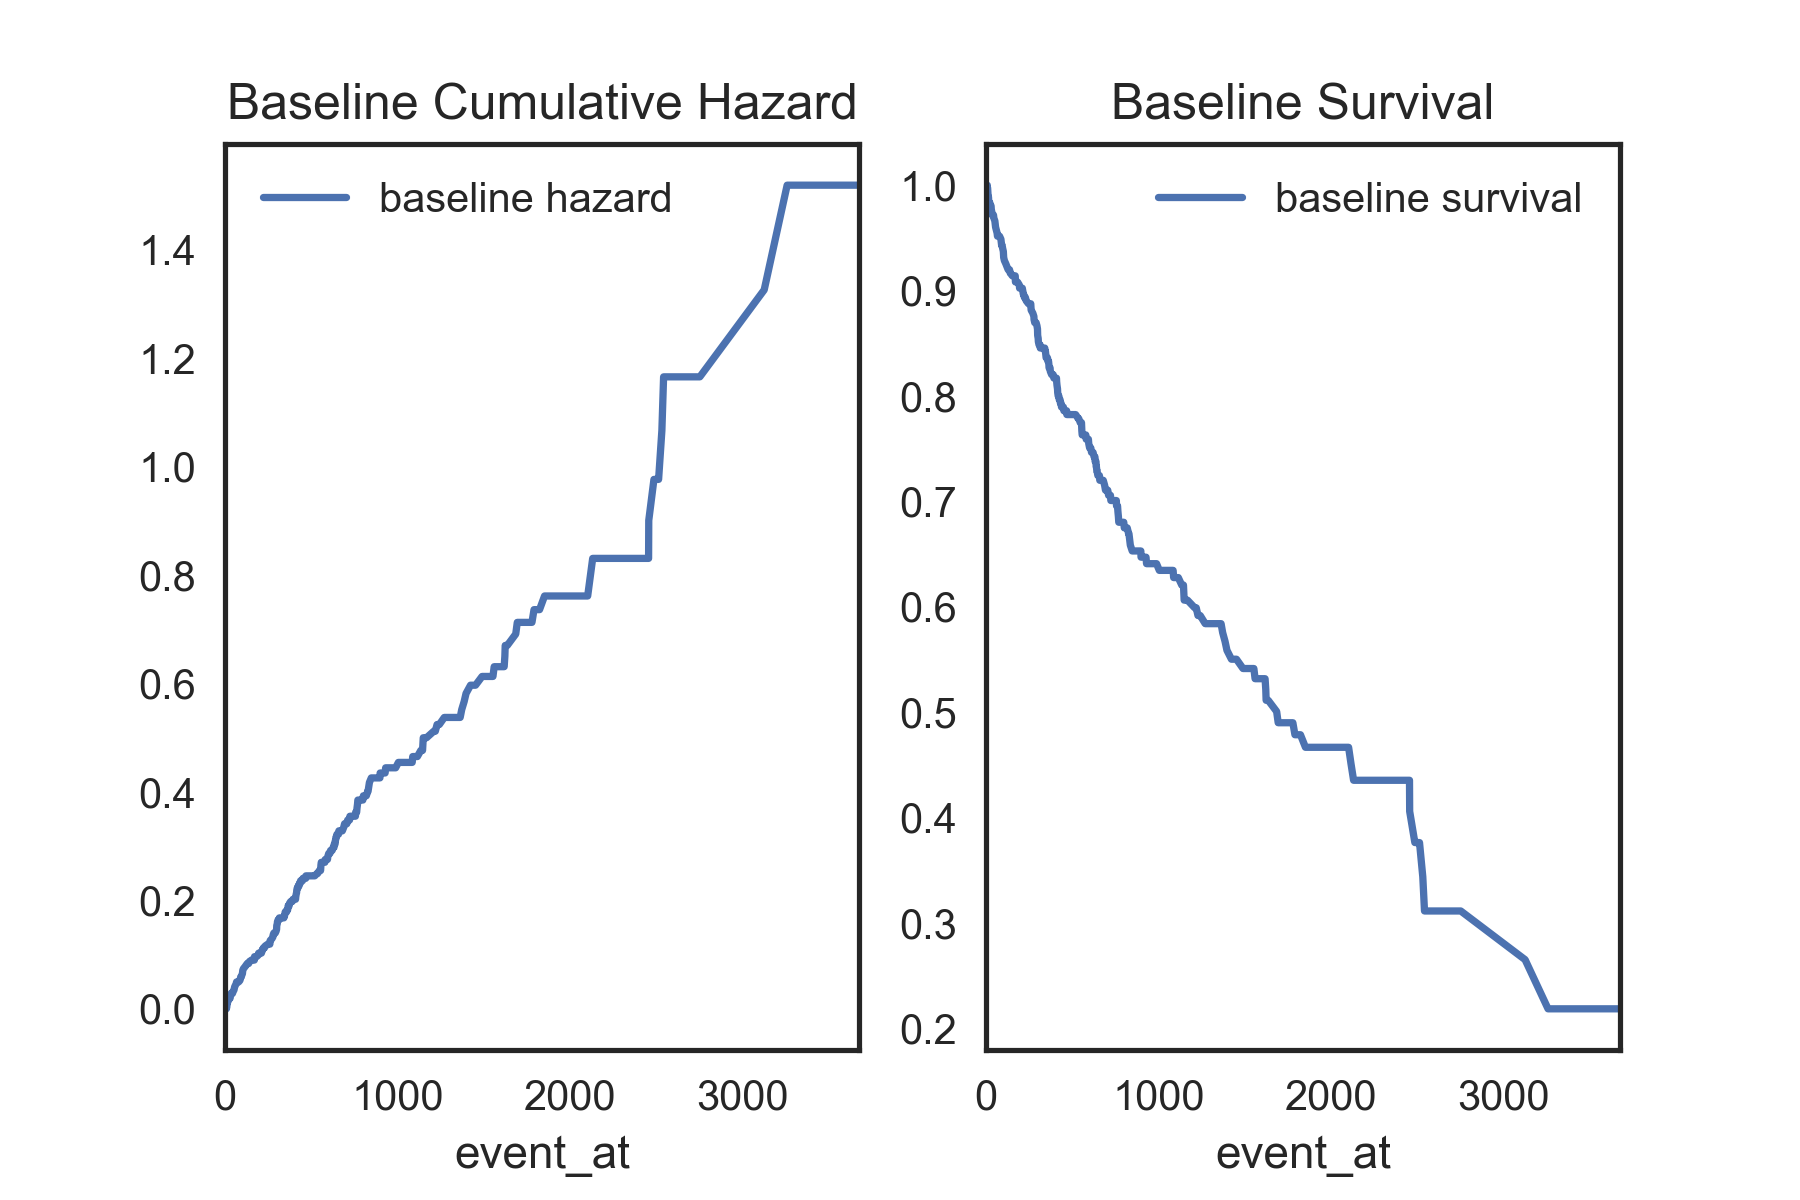
\includegraphics[width=0.75\textwidth]{survial_plot_one_mock_gene.png}
    \caption{The baseline cumulative hazard function for a mock gene transcript $ENSG00000000003$   The p-value for the transcript was $0.43$ with hazard coefficient of $-0.0057$ indicating that it is not a reliable prognostic marker of liver caner prognosis.}
    \label{fig:Baseline_hazard_and_survival}
\end{figure}
  		
	\subsection { Multiple hypothesis correction }
	
	\subsubsection {Estimating $\pi_0$ estimates on pvalues}
	
	Storey and Tibshirani \cite{storey2003statistical} provided the mathematical implementation for false positive discovery rate.  Using the implementation as discussed in the paper we calculated the $\pi_0$ estimates. Using the cublc spline fitting $\pi_0$ and  $\lambda$ values we calculated the  $\hat {\pi_0}$ for the p-values obtained from Cox model for each transcript as shown in figure~\ref{fig:estimate_pi}. The  $\hat {\pi_0}$  was estimated at $0.56$. 
\vspace{50cm} 
\begin{figure}
    \centering
     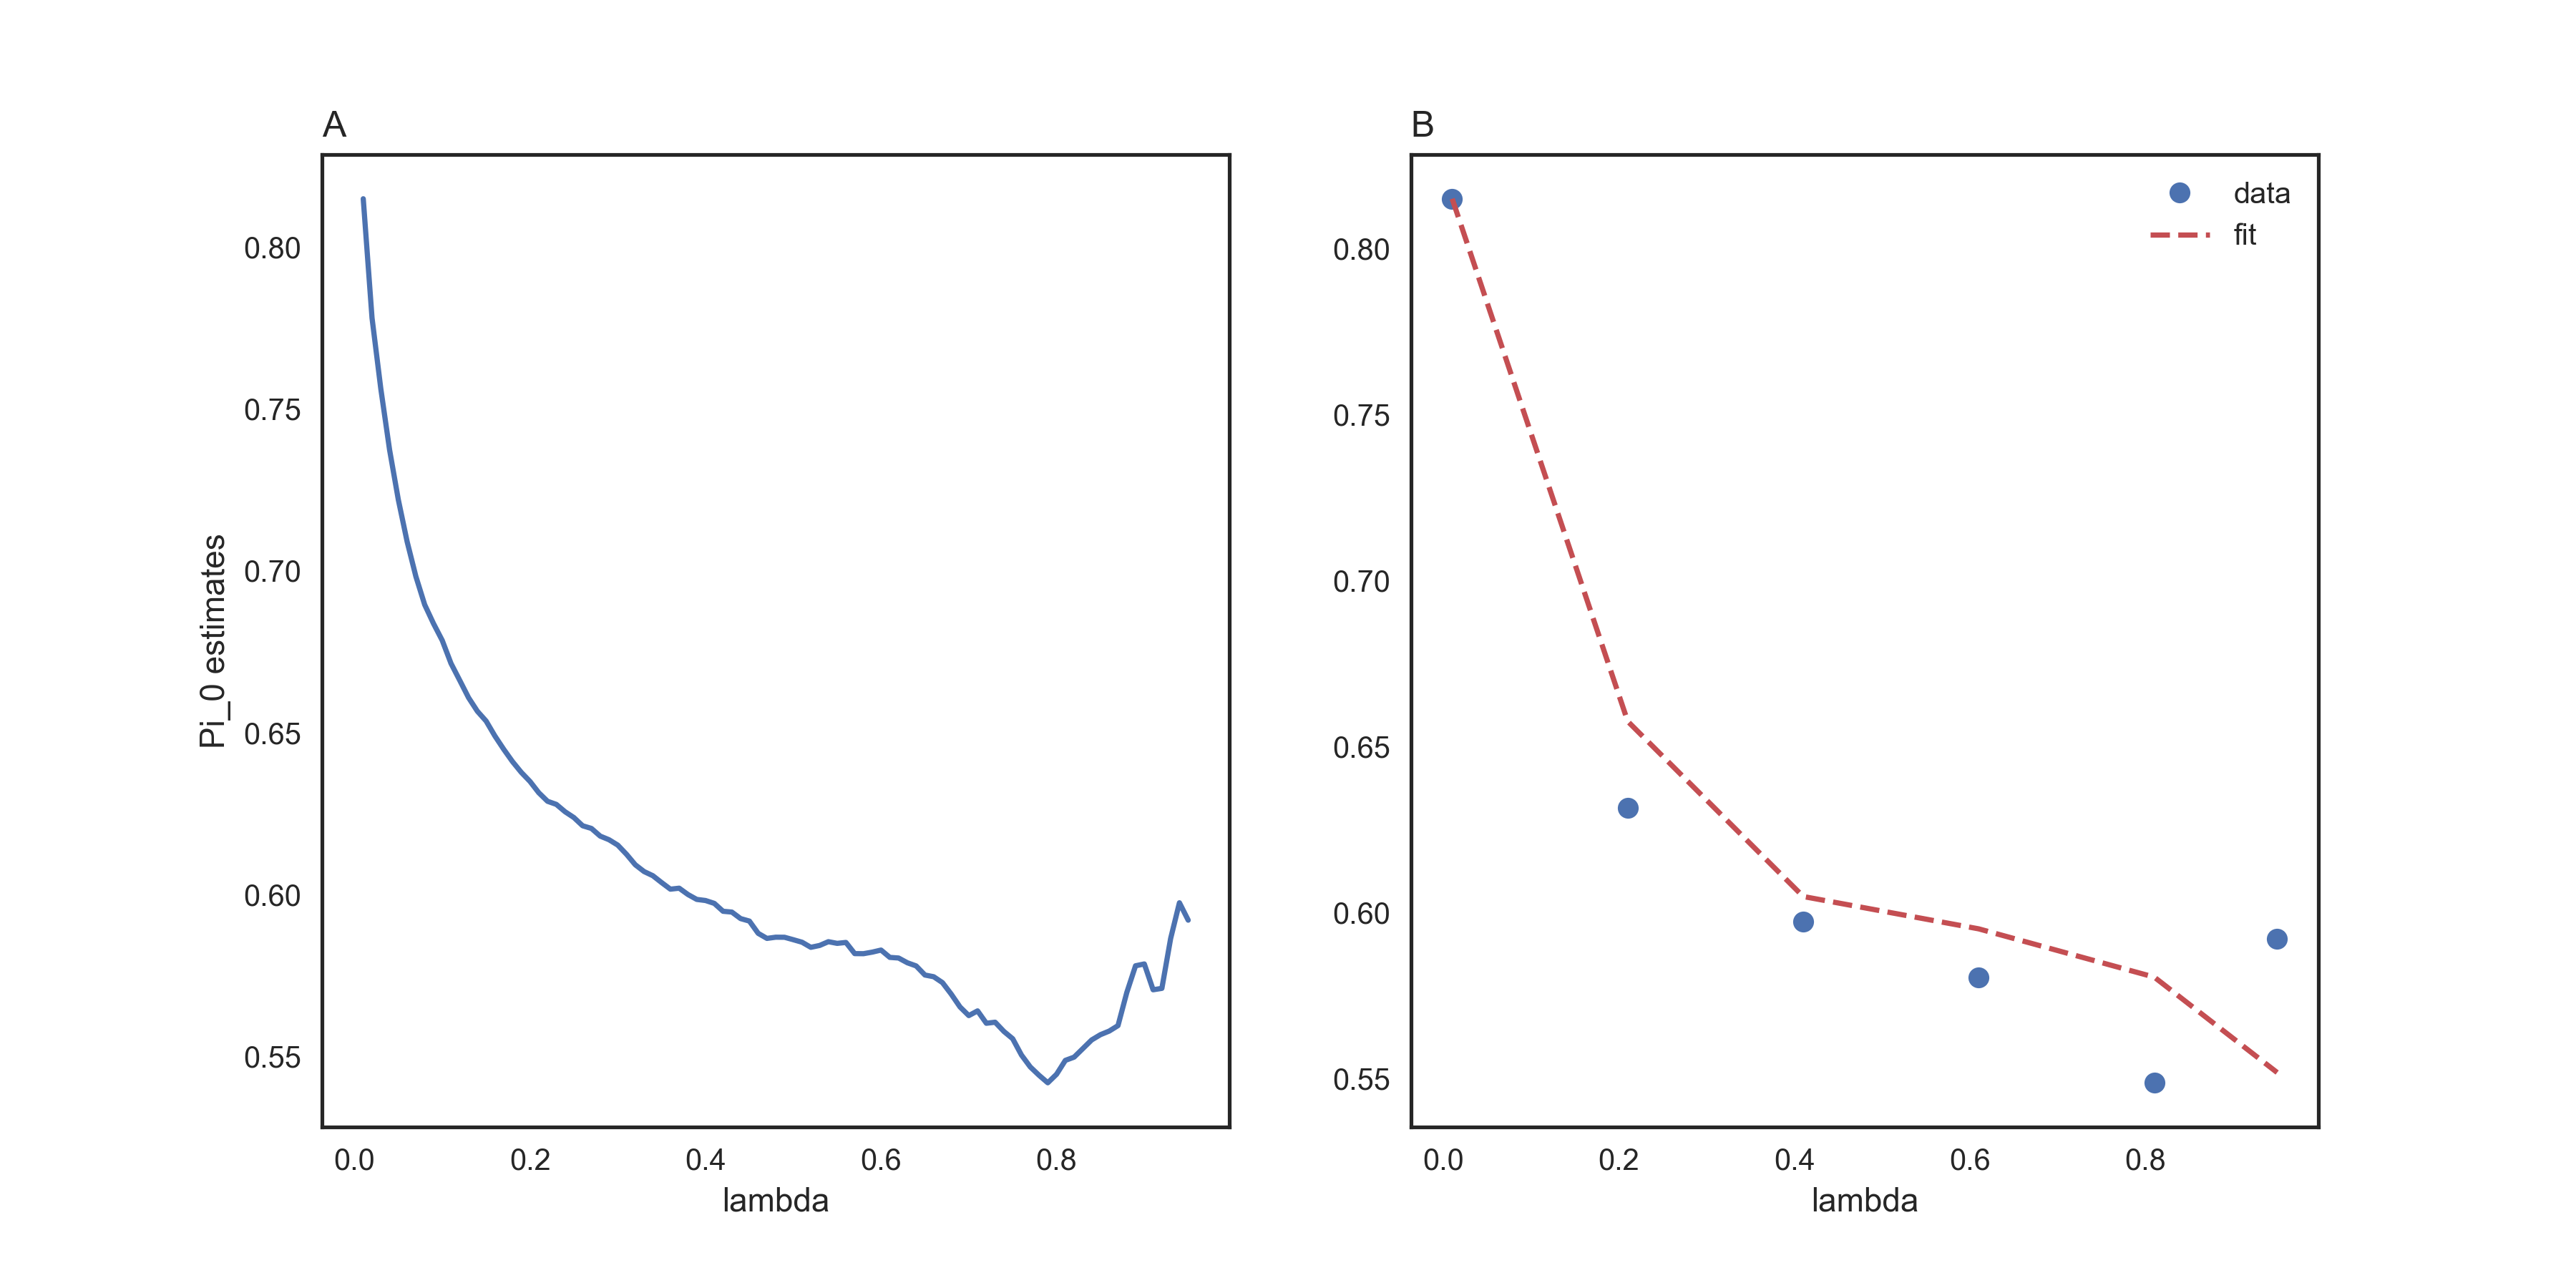
\includegraphics[width=\textwidth]{lambdaestimatescurvefitting.png}
    \caption{ A) $\pi_0$ estimates of $\lambda$  for $0.01$ to $0.95$ using the Storey and Tibshirani \cite{storey2003statistical} implementation in python. B) Cubic spline fitting to $\pi_0$  and $\lambda$ estimates. The blue points are subsets of real data and dotted lines are corresponding  fitted cublic spline   \tiny}
    \label{fig:estimate_pi}
\end{figure}

	\subsubsection {Estimation of q-values based on $\hat {\pi_0}$  values }
	 For each p-values of the transcript gene expression, a $\hat {\pi_0}$ $p_i$  was implemented in python in order to find the estimated q values for the  $i$th significant features using the equation as defined in Storey and Tibshirani \cite{storey2003statistical}. As shown in figure~\ref{fig:estimate_pi} we are able to control the false postive rates for p values calculated. We are able to find at least 4649 expressed gene transcript at $q$ $<$ $0.05$ . However considering the number of features tested we can further go to stricter cutoff such as $q < 0.01$ which would yield us 2464 gene transcript expression  as prognostic marker of liver cancer survival. 

	
\begin{figure}
\hspace*{-4cm}         
\centering
     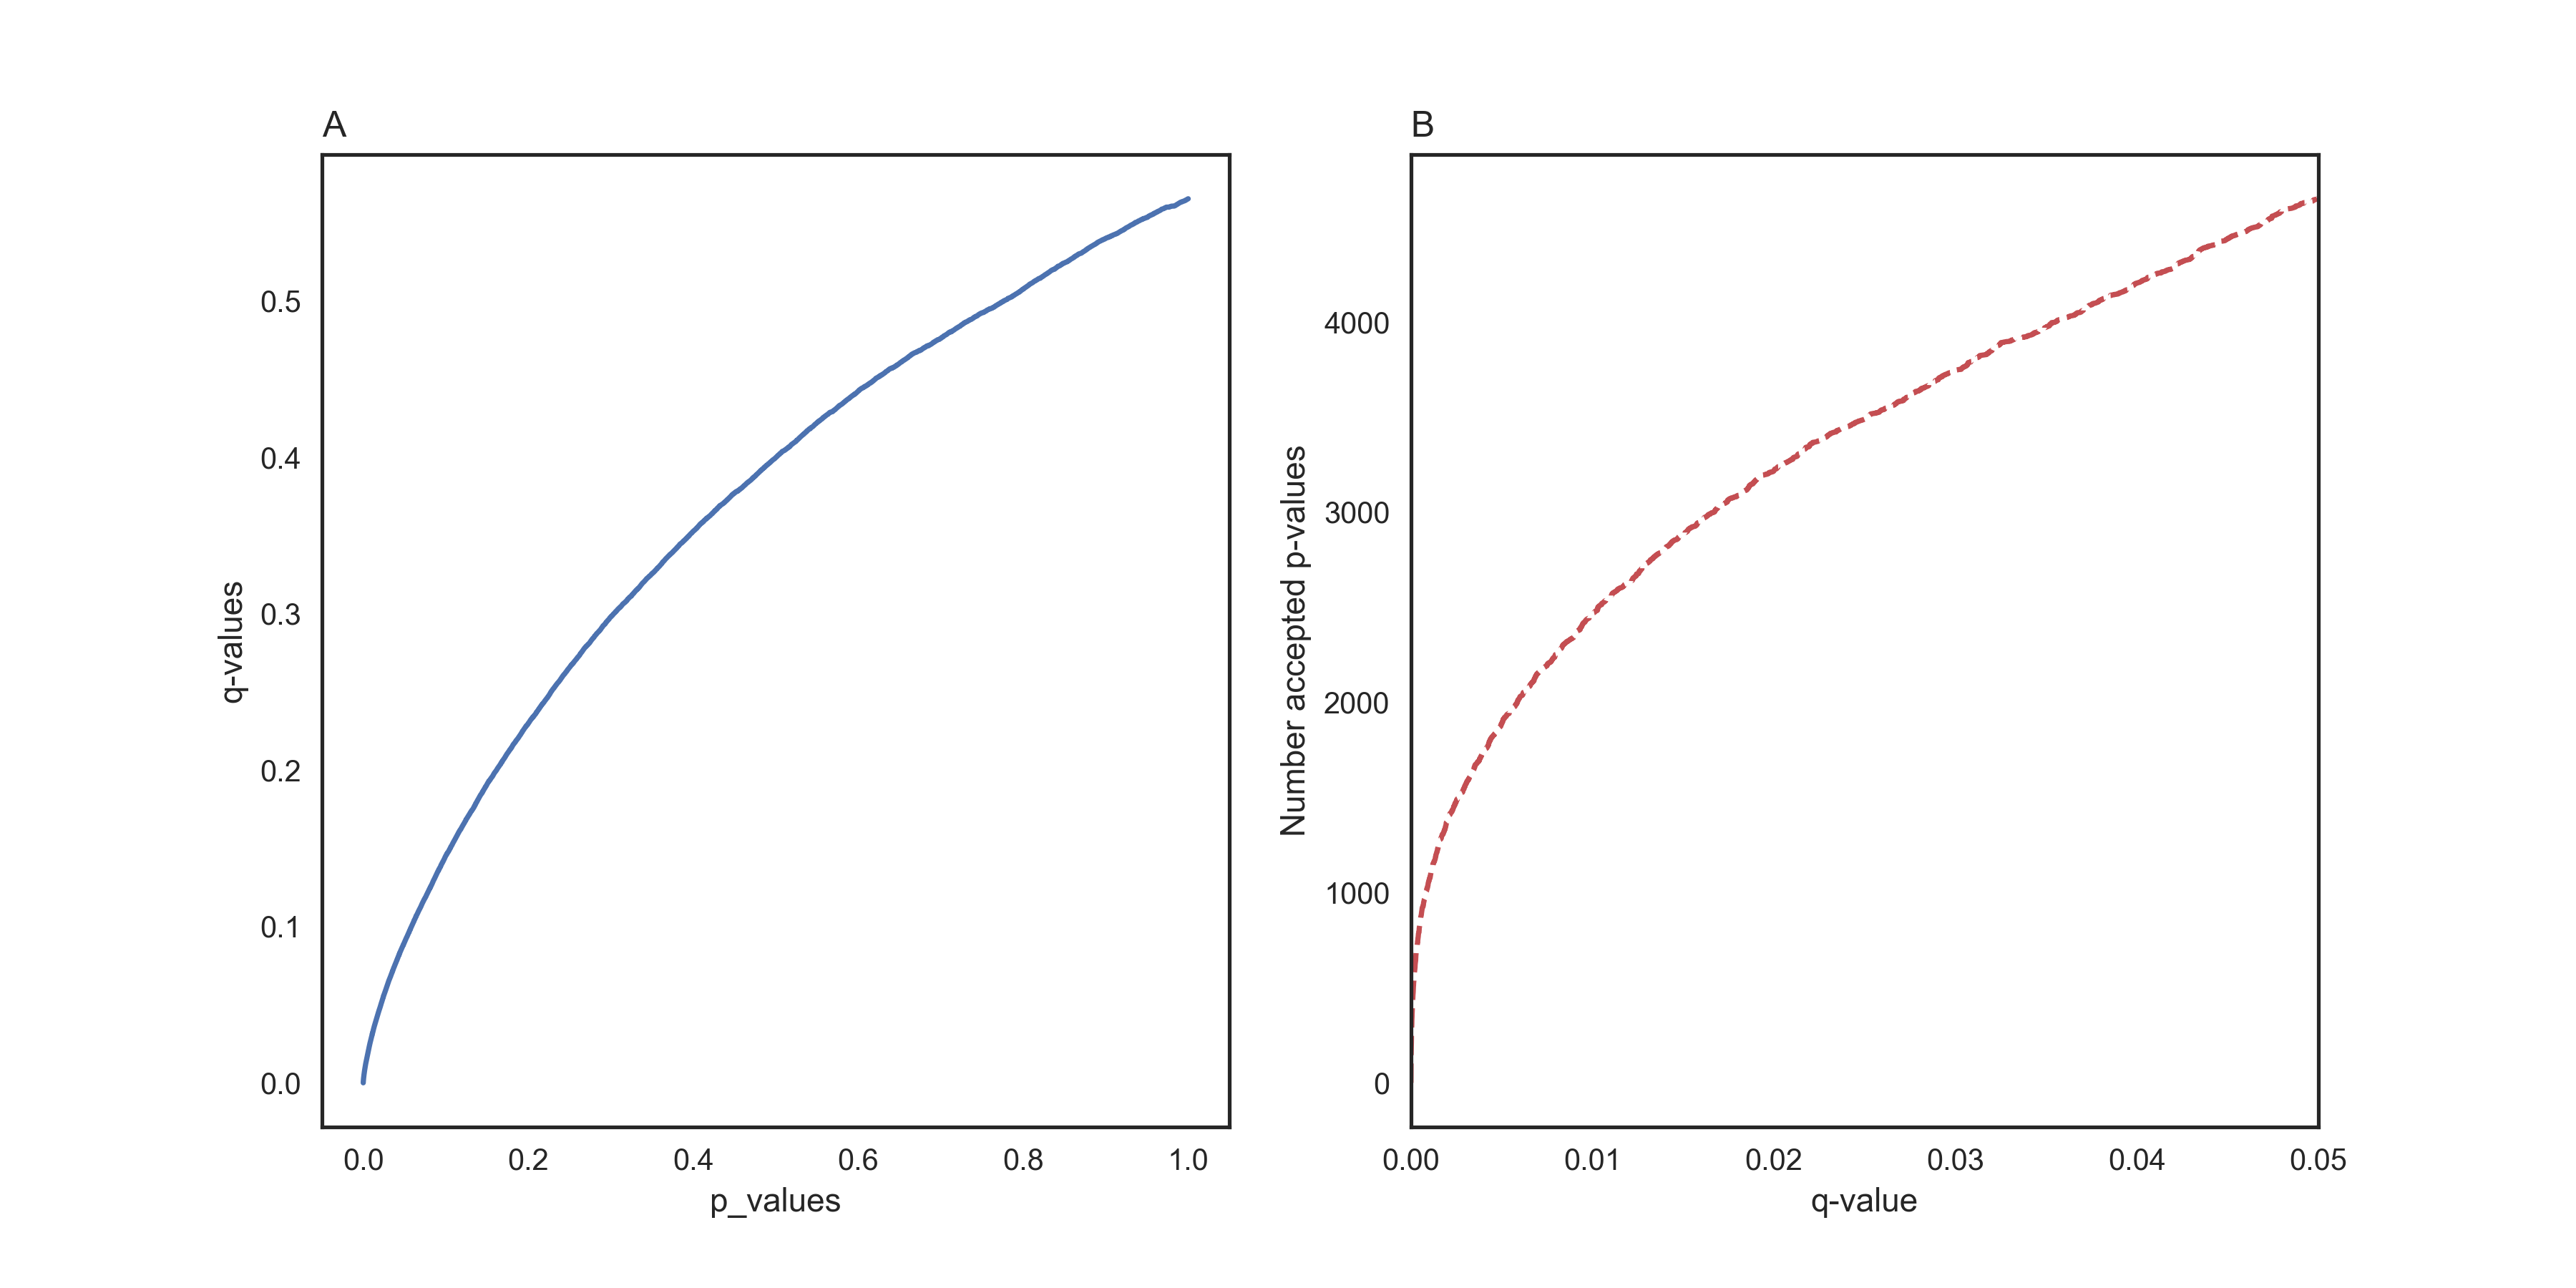
\includegraphics[width=1.57\textwidth]{comb.png}
    \caption{A) p VS q values for  different gene expression features. B) The number of $p$ values accepted at $q$ values $0.05$ . C) The number of $p$ values accepted at $q$ values $0.01$}
    \label{fig:animals}
\end{figure}



\newpage
\bibliographystyle{plain}
\bibliography{new_lib}

\end{document}
